\section{Projektorganisation}

Die Studierenden werden im Projekt 1 (pro1E) für den Studiengang Elektro- und Informati- onstechnik von drei Dozenten der Fachhochschule Nordwestschweiz (FHNW) unterstützt. Pascal Buchschacher informiert über Projektmanagement allgemein, Anita Gertiser vermittelt den Studenten die richtige Kommunikation innerhalb des Teams und Felix Jenni steht als Ansprechpartner für Fragen technischer Natur zur Verfügung.

Dieser Teil des Pflichtenhefts wurde erstellt, um den organisatorischen Teil des Projekt 1 abzudecken. Er zeigt die allgemeine Projektorganisation, die Planung, das Budget und die Risikoanalyse auf.
\subsection{Projektverantwortliche}

\subsection{Auftraggeber}
Auftraggeber des Projekts 1 ist Felix Jenni, Dozent an der Fachhochschule Nordwestschweiz.

\subsection{Teammitglieder}
Das Team 3 des Projekts 1 setzt sich aus sechs Studenten der Fachhochschule Nordwestschweiz, Hochschule für Technik in Brugg/Windisch zusammen. Frank Imhof (FI) ist der Projektleiter und verantwortlich für die Arbeiten und die Kommunikation mit dem Auftraggeber und den Fachdozenten. Unterstützt wird dieser vom stellvertretenden Projektleiter \newline Pascal Puschmann (PP). Die übrigen Mitglieder sind Michel Alt (MA), Lars Bachmann (LB), Roni Fischer(RB) und Christoph Kuhn(CK). Jeder von ihnen studiert Elektro- und Informationstechnik im ersten Semester, mit Ausnahme von Christoph Kuhn, der gleichzeitig das Projekt 3 absolviert.

\subsection{Organigramm}
\begin{figure}[H]
	\centering
	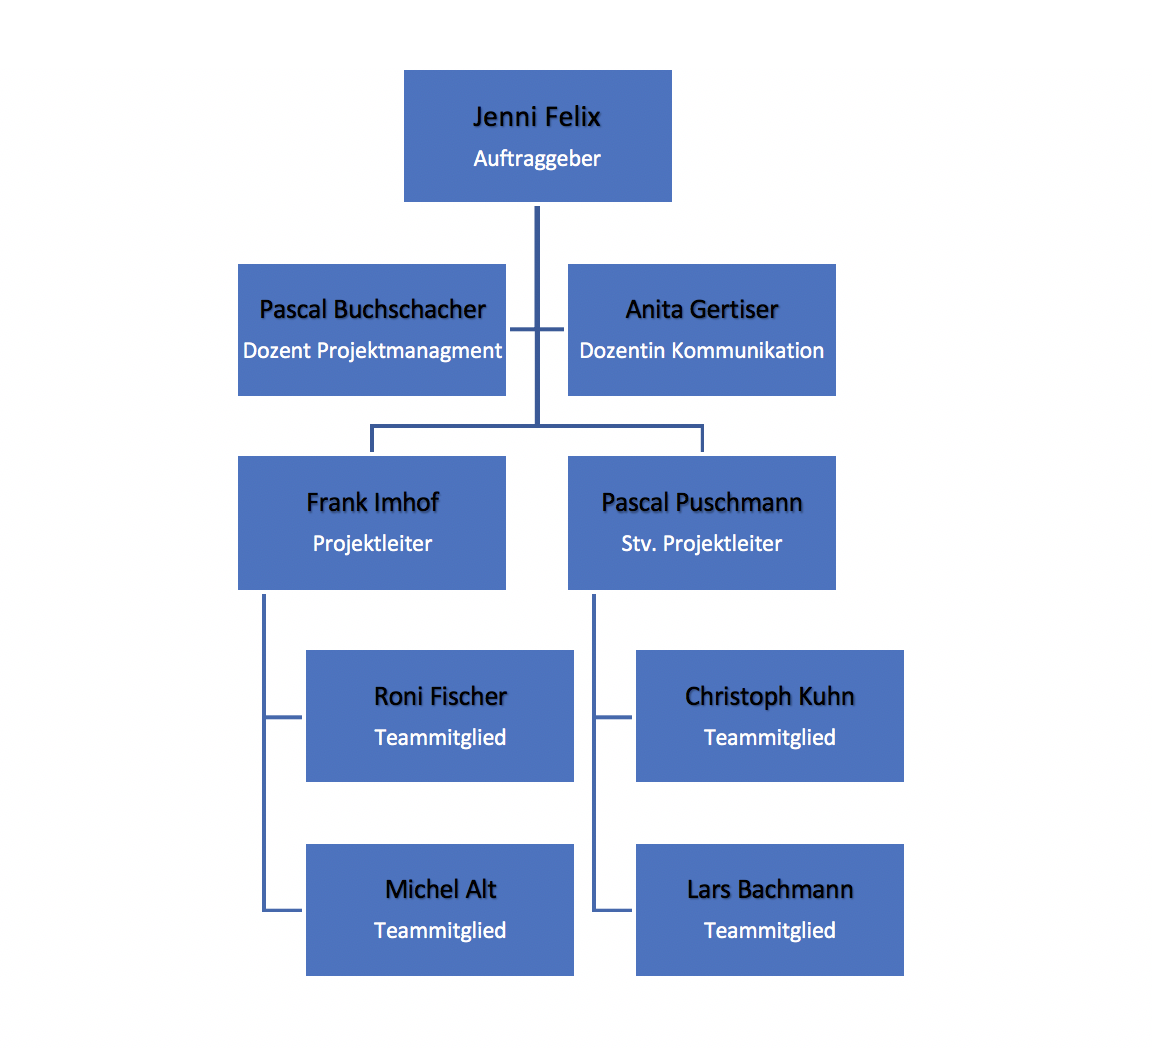
\includegraphics[width=10cm]{Organi.png}
	\label{fig:Organigramm}
\end{figure}
